\documentclass[11pt,letterpaper]{article}

\usepackage{hyperref}
\usepackage{graphicx}
\usepackage{fancybox}
\usepackage[utf8]{inputenc}
\usepackage{epsfig,graphicx}
\usepackage{multicol,pst-plot}
\usepackage{pstricks}
\usepackage{amsmath}
\usepackage{amsfonts}
\usepackage{amssymb}
\usepackage{eucal}
\usepackage{upgreek}
\usepackage[left=2cm,right=2cm,top=2cm,bottom=1cm]{geometry}
\usepackage{tcolorbox}
\usepackage{import}
\pagestyle{empty}
\DeclareMathOperator{\tr}{Tr}
\renewcommand{\sp}[1]{$${\begin{split}#1\end{split}}$$}

\usepackage{lipsum}
\usepackage{mdframed}
\usepackage{listings}
\usepackage{color}

% Margins
% \topmargin=-0.45in
\evensidemargin=0in
\oddsidemargin=0in
\textwidth=6.5in
\textheight=9.0in
\headsep=0.25in

% \title{ Chemistry Notes}
% \author{ Gurmukh Singh }
% \date{\today}

 % The problem environment introduced.                                     
\newenvironment{problem}[2][Problem]                                  
        {\begin{tcolorbox}[colback=white,colframe=gray!50,title=#1 #2]}
        {\end{tcolorbox}}
        % {\begin{mdframed}[backgroundcolor=gray!20] \textbf{#1 #2} \\}
        % {\end{mdframed}}
% Define solution environment
\newenvironment{solution}                      
        {\begin{mdframed}\textit{Solution:} \\}
        {\end{mdframed}}
% Define an environments for proofs
\newenvironment{myproof} 
        {\textit{Proof:}}                                   
        {\begin{flushright} Q.E.D. \end{flushright}}
% Define a theorem environment and a notation one too
\newenvironment{mytheorem}                    
        {\begin{mdframed}\textbf{Theorem:} \\}
        {\end{mdframed}}
\newenvironment{notation}                      
        {\begin{mdframed}\textit{Notation:} \\}
        {\end{mdframed}}
% A new example wouldnt so any harm either...  
\newenvironment{example}                             
        {\textit{Example:}\\}
	{}
%I sholud be ashamed to forget the definition environment
\newenvironment{definition}
	{\begin{mdframed}$\underline{\textit{Def}^\textit{n}:} $\\}
	{\end{mdframed}}
%Corollary envvvvvvvvv
\newenvironment{corollary}
	{\textbf{Corrolary:}\\}

\pagestyle{empty}

\begin{document}

\begin{center}
  \Huge{Statistics Notes}\\
  \vspace{0.25cm}
  \small{Gurmukh Singh}
\end{center}

\vspace{-1.75cm}

\begin{flushright}
  Instructor: \\ Mrs. Neha
\end{flushright}

\vspace{-1.3cm}

\begin{flushleft}
  B.Tech. CSE
\end{flushleft}

\rule{15.5cm}{0.1mm}%{\linewidth}{0.1mm}

% Optional TOC
\tableofcontents
\pagebreak

%--Paper--

\begin{mdframed}[backgroundcolor=gray!20]
   ``All models are wrong, but some of them are useful''
   \begin{flushright}
     $\sim$ George Box
   \end{flushright}
\end{mdframed}

\section{Measures of Central Tendency}
\begin{enumerate}
  \item Mean
  \item Median
  \item Mode
\end{enumerate}

\subsection{Mean}
It is the ratio of sum of all the observations to the total number of observations.
let $x_1, x_2, \dots, x_n$ be all the observations. then:
\[
  \overline{x} =\frac{\sum_{i=1}^n x_i}{n}
\]

\subsubsection{Properties of Mean}
\begin{itemize}
  \item The sum of deviation of observations from mean is always zero
  \item the sum of square of deviations of observations is minimum as compared to any other measure.
  \item suppose there are two sequences:
    \[
      \begin{tabular}{c|c|c}
        & Series 1 & Series 2 \\ 
        Number of observations & $n_1$ & $n_2$ \\ 
        mean of the observations & $\overline{x}_1 $& $\overline{x}_2$
      \end{tabular} 
    \]
    then
    \[
      \overline{x} = \frac{n_1x_1+n_2x_2}{n_1+n_2}
    \]
\end{itemize}

\begin{problem}1
  If there are 5 and 8 number of observations of 2 series with mean 15 and 18, find the combined mean
\end{problem}

\begin{solution}
  We can get the solution by taking the weighted mean of the two sequences. \\ 
  so the required mean is : 
  \[
    \frac{5 \times 15 + 8 \times 18}{5+8}
  \]
  \[
    = \frac{75 + 144}{13}
  \]
  \[
    = \frac{219}{13}
  \]
  \[
    = 16.846154
  \]
\end{solution}

\begin{problem}2
  $$
   \begin{tabular}{c c}
     Class & frequency \\ 
   0-10 & 3 \\ 
   10-20 & 5\\ 
   20-30 & 7\\ 
   30-40 & 4\\ 
   40-50 & 1\\ 
   \end{tabular}
  $$
\end{problem}

\begin{solution}
  change of origin:
  $$
   \begin{tabular}{c c c c c }
     Class & frequency & X & d=X-A & f$\cdot $d\\ 
     0-10 & 3 & 5 & -20 &  \\ 
     10-20 & 5 & 15 & -10  & \\ 
     20-30 & 7 & 25 & 0 & \\ 
     30-40 & 4 & 35 & 10 & \\ 
     40-50 & 1 & 45 & 20 & \\ 
   \end{tabular}
  $$
  \[
    \overline{x} = A + \frac{\sum fd}{n}
  \]

  change of scale
  $$
   \begin{tabular}{c c c c c }
     Class & frequency & X & d=X/n & f$\cdot $d\\ 
     0-10 & 3 & 1 & -20 &  \\ 
     10-20 & 5 & 3 & -10  & \\ 
     20-30 & 7 & 5 & 0 & \\ 
     30-40 & 4 & 7 & 10 & \\ 
     40-50 & 1 & 9 & 20 & \\ 
   \end{tabular}
  $$
  \[
    \overline{x} = A + \frac{\sum fd}{n}
  \]
\end{solution}

\subsection{Median}
Steps to find Median in case of Discrete and continuous data:

\begin{enumerate}
  \item Arrangement of data
  \item if $n$ is odd then the median is the $ \frac{n+1}{2}$th term
  \item if $n$ is even then the median is the mean of the $\frac{n}{2}$th term and $\frac{n}{2}+1$th term
\end{enumerate}
\begin{problem}3
   find the median for the data : 
   \begin{enumerate}
      \item 9,9,10,10,12,13,15
      \item 9,9,10,10,12,13,14,15
   \end{enumerate}
\end{problem}

\begin{solution}
  \begin{enumerate}
    \item 9,9,10,10,12,13,15 has 7 elements. Therefore our median will be the 4th term in the arranged order\\
      $ \therefore Median = 10 $
    \item 9,9,10,10,12,13,14,15 has 8 elements. Therefore our median will be the mean of the 4th and 5th terms. \\
      $\therefore Median = \frac{10+12}{2}= 11$
  \end{enumerate}
\end{solution}

\begin{problem} 4
  Finding the median of discrete data. 
  \begin{center}
    \begin{tabular}{c|c|c}
      X & f & cf(cumulative frequency)\\
      \hline
      1 & 5 & 5\\ 
      2 & 8 & 13\\ 
      3 & 9 & 22\\ 
      \textbf{4} & \textbf{12} & \textbf{34}\\ 
      5 & 6 & 40\\ 
      6 & 7 & 47\\ 
      7 & 4 & 51\\ 
      \hline
      Total & 51 \\
    \end{tabular}
  \end{center}

  find the value of $x$ which has cumulative frequency just greater than $\frac{n}{2}$
\end{problem}

In case of continuous data:
\[
  Median = l + \frac{\left( \frac{n}{2} - cf \right)h}{f}
\]
where cf is the cumulative frequency and f is the frequency of the chosen class, $h$ is the class size

\subsection{Mode}
The observation which occurs the most is called the mode of the data. \\
In more general terms, the most probable observation in a dataset is the mode of the data. 

\begin{problem}5
  Find mode for the following data:
  10,11,15,18,18,18,15,10,18,20
\end{problem}

\begin{problem}6
  Find the mean, median and mode for the following data
  \begin{center}
    \begin{tabular}{c|c}
      CI & f \\
      \hline
      0-10 & 3 \\
      10-20 & 5 \\ 
      20-30 & 7 \\ 
      30-40 & 2\\ 
      40-50 & 1 \\ 
      \hline
      Total & 51 \\
    \end{tabular}
  \end{center}
\end{problem}
\textbf{How to find the mode for continuous data}
\begin{enumerate}
  \item Find the modal class which is having the maximum frequency.
  \item based on that input the values into the following formulae:
    \[
      mode = l + h \left( \frac{f_1 - f_2}{2f_1-f_0-f_2} \right)
    \]
\end{enumerate}
\subsection{The interconnection between the measures of central tendency}
\[
  Mode = 3 Median - 2 Mean
\]

\subsection{Geometric and Harmonic mean}
\begin{definition}
   Geometric mean is defined as the $n$th root of the product of $n$ observations\\
   Mathematically:
   \[
     GM = \sqrt[n]{\prod_{i=0}^n x_i}
   \]
\end{definition}

\begin{problem}7
   Find the Geometric Mean for the values 2,4,8
\end{problem}

\begin{definition}
   Harmonic mean is defined as the reciprocal of arithemetic mean of the reciprocal of all the observations
   \[
      HM = \frac{n}{\sum_{i=1}^{n} \frac{1}{x_i}}
   \]
\end{definition}

\begin{mytheorem}
   The following inequality is always true:
   \[
      AM \geq GM \geq HM
   \]
\end{mytheorem}

\subsection{Histogram}
Histogram can also be used to compute the value of mode. 

\subsection{Ogive}
Ogives are used to compute the value of median. 
They are nothing but graphs of cumulative distribution functions. \\ 
The point of intersection of two ogives gives the median. 

\subsection{Quartiles}
Quartiles are the values which divide the dataset into 4 equal parts. These points are called $ Q_1, Q_2, Q_3$. 

\[
  Q_1 = l + \frac{\left( \frac{n}{4} - cf \right)h}{f}
\]

\[
  Q_2 = l + \frac{\left( \frac{n}{2} - cf \right)h}{f}
\]

\[
  Q_3 = l + \frac{\left( \frac{3n}{4} - cf \right)h}{f}
\]
\subsection{Deciles}
Deciles are the values which divide the dataset into 10 equal parts. 

\subsection{Percentiles}
Percentiles are the values which divide the dataset into 100 equal parts. 

To find the $x$th percentile we can use the following formulae:

\[
  p_{x} =l + \frac{\left( \frac{x n}{100} - cf \right)h}{f} 
\]

\section{Measures of Spread/Dispersion}

Measures of spread are a numerical quantity to signify the variation in the observations.\\
Dispersion means the scatterment of observations. \\
There are a number of ways to get a gist of the Dispersion. 

\begin{enumerate}
  \item Range: it is the difference between the maximum and minimum value of the dataset. 
  \item Quartile Deviation: It is equal to $\frac{Q_3-Q_1}{2}$
  \item Mean Deviation: It is the arithemetic mean of absolute value of deviation of observations from average. 
    \begin{align*}
      MD &= \frac{\sum \lvert x - \overline{x} \rvert}{n} ( Discrete )\\
         &=  \frac{\sum f \lvert x - \overline{x} \rvert}{N} ( Continuous )
    \end{align*}
  \item Standard deviation: It is the positive squareroot of arithemetic mean of square of deviation of observations 
    from mean. It is denoted by $\sigma$. This is applicable when your mean is an integer.
    \[
      \sigma = \sqrt{\frac{\sum (x - \overline{x})^2}{n}} ( helpful\ when\ mean\ is\ integral )
    \]

    \[
      \sigma = \sqrt{\frac{1}{n}\left( \sum x^2 - \frac{(\sum x)^2}{n}\right)} ( helpful\ when\ mean\ is\ non-integral\ and\ x\ is\ small )
    \]
    This is an alternate derivation of the formulae $V = E[X^2]-E[X]^2$

    \[
      d = x-a; 
      \sigma = \sqrt{\frac{1}{n}\left( \sum d^2 - \frac{(\sum d)^2}{n}\right)} ( helpful\ when\ mean\ is\ non-integral\ and\ x\ is\ large )
    \]
  \item Variance: It is the square of standard deviation. 
    \[
      V = \sigma^2 
    \]
\end{enumerate}

\subsection{Coefficient of variation}
It is another way of measuring the spread. It is analogous to standard deviation with respect to the mean. 
\[
  CV = \frac{\sigma}{\overline{X}} \times 100
\]
Suppose there are two sequences with $n_1$ and $n_2$ observations. \\ 
$\overline{x}_1$ and $\overline{x}_2$ are their means. \\ 

their combined variance will be: 
\[
  \sigma^2 = \frac{2}{n_2 + n_2} [n_1(\sigma_1^2 + d_1^2) + n_2(\sigma_2^2 + d_2^2)]
\]
where $d_i = \overline{x}_i - \overline{x}$. here $ \overline{x}$ is the combined mean of the series. 

\subsection{Skewness and Kurtosis}

While studying a distribution we can calculate the measures of central tendency and the measures of spread. 
However even this information is not enough to determine the behavior of the randow variable distribution. 
In order to further narrow down in the analysis of the beha vior of the variable we study the skewness of the distribution. 

A distribution is called skewed if: 
\begin{itemize}
  \item The Measures of central tendencies do not coincide. 
  \item The curve does not follow gaussian nature. 
  \item The quartiles are not equidistant from the median. 
  \item Some of the positive deviations from median is not equal to the sum of negative deviations from the median. 
\end{itemize}


\includegraphics[width = \textwidth]{figs/Pasted image.png}

There can be two types of skewness: 
\begin{enumerate}
  \item Positive skewness (Right skewed)
  \item Negative skewness (Left skewed)
\end{enumerate}

\[
  S_k = Mean - Mode
  \begin{cases}
    = 0 & if\ data\ is\ symmetrical\\
    > 0 & if\ data\ is\ positively\ skewed\\
    < 0 & if\ data\ is\ negatively\ skewed
  \end{cases}
\]

\subsubsection{Positive skewness}
In this most of the values lie to the right to the peak. 

one way to determine this is that $mode > median > mean$ 


\subsubsection{Negative skewness}
In this most of the values lie to the left to the peak. 

one way to determine this is that $mode < median < mean$ 

\subsubsection{Moments}
Arithemetic mean of various powers of deviation of observation from mean. 

\[
  \mu_r = \frac{\sum(x-\overline{x})^r}{n}
\]

\begin{enumerate}
  \item $\mu_1 = 0$
  \item $\mu_2 = $ variance
  \item $\mu_3 = $ skewness
  \item $\mu_4 = $ kurtosis
\end{enumerate}

\subsubsection{Coefficient of skewness:}
\[
  \beta_1 = \frac{\mu_3^2}{\mu_2^3}
\]

\[
  \gamma_1 = \frac{\mu_3}{(\sqrt{\mu_2})^3}
\]
if $\gamma_1 = 0$ the data is symmetrical. \\
if $\gamma_1 > 0$ the data is right skewed. \\
if $\gamma_1 < 0$ the data is left skewed. \\

\subsubsection{Kurtosis}

It measures the flatness or peakness of the distribution. 

\vspace{1cm}

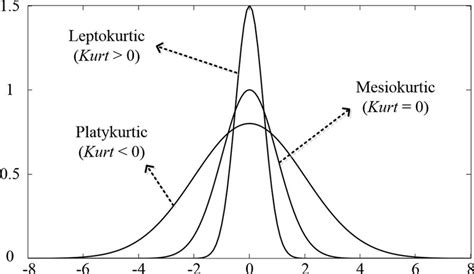
\includegraphics[width = \textwidth]{figs/Pasted image (2).png}

\[
  \beta_2 = \frac{\mu_4 }{(\mu_2)^2}
\]


\[
  \gamma_2 = \beta_2 - 3
\]

\[
  Distribution = \begin{cases}
    Mesokurtic,\ if\ \gamma_2 = 0\\
    Leptokurtic,\ if\ \gamma_2 > 0\\
    Platykurtic,\ if\ \gamma_2 < 0
  \end{cases}
\]

\section{Probability}
Probability is the measure of belief that a certain event will occur. 
\subsection{Prerequisites}

\begin{definition}
  Trial:\\
Suppose an experiment is repeated under identical and homogeneous conditions does not give unique result
but may result in one of several possible outcomes. The experiment is known as a random experiment or a Trial.
\end{definition}

For example: the toss of a coin.\\
The outcome of a Trial is known as an \textbf{event. }

\begin{definition}
Exhaustive events:\\
The set of all the simple events that can occur in a trial are called exhaustive events. 
The cardinality of the sample space can be found out using basic Combinatorics.
\end{definition}

\begin{problem}8
  What would be the sample space of the experiment in which 2 coins are tossed together.
\end{problem}

\begin{solution}
  \{HH,HT,TH,TT\}
\end{solution}

\begin{definition}
Mutually Exclusive Events:\\
Events are mutually exclusive if no two or more than 2 events occur simultaneously in the same trial
\end{definition}

Mathematically, two events $E$ and $F$ are mutually exclusive $\iff E \cap F = \phi$

\begin{definition}
Favourable events:\\
The number of simple events favourable to the happening of an event. 
\end{definition}

\begin{definition}
Equally likely events:\\
This means that events have equal chances of occurence.
\end{definition}

\begin{definition}
Independent events:\\
Two events are called Independent if the occurence of one event does not influence the occurence of the other. 

Mathematically, Two events are independent if
\[
  P(E \cup F) = P(E) \times P(F)
\]
\end{definition}

\subsection{Definition of Probability}
\subsubsection{Mathematical or Empirical Probability}

The probability of an event $E$ is 
\[
  P(E) = \frac{number\ of\ simple\ events\ favourable\ to\ E}{Total\ number\ of\ simple\ events}
\]

Suppose there are total of $n$ number of events and the number of events favourable for a certain event are $m$. then the probability will be $\frac{m}{n}$.

Then the number of events unfavourable to the same event is $n-m$ and the probability will be $\frac{n-m}{n}$

Axiomatically:
\[
  P(E) = 1- P(\overline{E})
\]

and 

\[
  0 \leq P(E) \leq 1 \ \forall E \subset \Omega
\]

\subsubsection{Statistical Probability}
The probability of an event $E$ is 
\[
  P(E) = \frac{number\ of\ simple\ events\ favourable\ to\ E}{Total\ number\ of\ simple\ events}
\]

\subsubsection{Axiomatic Probability}
Consider a sample space $S$. The probability is a function that assigns a non-negative value to every event, say $A$ denoted by $P(A)$ is called the probability of an event $A$ if it satisfies the following properties. 
\begin{enumerate}
  \item $P(A) \in [0,1] \forall A \subset S$
  \item $P(S) = 1$
  \item $P(\bigcup_{i=1}^n A_i) = \sum_{i=1}^n P(A_i)$ where each $A_i$ is a mutually exclusive event
\end{enumerate}

\subsection{Addition law of Probability}
If $A$ and $B$ are two events and are not mutually exclusive, so : 
\[
  P(A \cup B) = P(A) + P(B) - P(A \cap B)
\]

\subsection{Multiplication Law of Probability}
\[
  P(A\cup B) = P(A) \cdot P( B \vert A )
\]

if $A$ and $B$ are independent then $ P( B \vert A ) = P(B)$ and 

\[
  P(A\cup B) = P(A) \cdot P( B )
\]

\subsection{Bayes Theorem}
If $E_1, E_2, E_3 \dots E_n$ are $n$ mutually exclusive events with $P(E_i) > 0 \forall i$ then for any event $A$ 
which is a subset of $\bigcup_{i=1}^n E_i$ 

\[
  P(E_1 \vert A) = \frac{P(E_1) P(A \vert E_1)}{\sum_{i=1}^n{P(E_i) P(A \vert E_i)}}
\]

Here $P(E_i \vert A)$ is called Posterior Probability.

\begin{problem}8
  A class consists of 5 girls and 7 boys. If a comittee of 3 is to be chosen at random what is the probability that 
  \begin{enumerate}
    \item 3 boys are selected\hfill (Ans = 0.159)
    \item exactly 2 girls are selected\hfill (Ans = 0.318)
  \end{enumerate}
\end{problem}
\begin{solution}
  \begin{enumerate}
    \item 
    \item 
  \end{enumerate}
\end{solution}

\subsection{Randow Variables}
Axiomatically a Random variable is a variable which takes values at random.
A random variable is a variable $X$ that assigns a real number for each and every outcome. 

For example, the number of heads in two tosses of a coin.

There are two types of Random variable:
\begin{enumerate}
  \item Discrete Random Variable: \\
    A random variable which takes countably many values. 
  \item Continuous Random Variable: \\ 
    A Random variable which takes uncountably many values.
\end{enumerate}

There are two types of probability functios: 
\begin{enumerate}
  \item Probability mass functions: \\
    The function is said to be a PMF if : 
    \begin{enumerate}
      \item $ 0 \leq P(X) \leq 1 $ 
      \item $\displaystyle \sum_{x \in \Omega} P(X) = 1 $ 
    \end{enumerate}
  \item Probability density functions:\\
    It gives a measure of how likely the variable is to lie in the neighbourhood of a point.
    The function $f_X(x)$ of the numeric values of a continuous randow variable is said to be a PDF if it satisfies:
    \begin{enumerate}
      \item $ f_X(x) \geq 0 \forall x$ 
      \item $\displaystyle \int_{-\infty}^\infty f_X(x) = 1$ 
      \item $\displaystyle P(a<x<b) = \int_a^b f_X(x) dx$
    \end{enumerate}
\end{enumerate}

\begin{problem}9
  A coin is tossed 3 number of times. Lets say $X$ be the number of times Head appears.
\end{problem}

\begin{solution}
  \begin{center}
  % \[
  %   \begin{tabular}{|c|c|c|c|c|}
  %     \rule
  %     $X$ & 0 & 1 & 2 & 3 \\
  %     \rule
  %     $f_X(x)$ & \frac{1}{8} & \frac{3}{8} & \frac{3}{8} &\frac{1}{8}
  %     \rule
  %   \end{tabular}
  % \]
  \end{center}
\end{solution}

\begin{problem}{10}
  A shipment of 8 microcomputers to a retailer outlet contains 3 defectives. 
  if a school makes a random purchase of 2 computers find the probability distribution for the number of defectives. 
\end{problem}

\begin{problem}{11}
  In an experiment of tossing 3 coins, obtain the probability distribution of: 
  \begin{enumerate}
    \item $X$ denotes the number of heads
    \item $Y$ denotes number of head runs
    \item $Z$ the number of successive heads
    \item $X+Y$ 
    \item $XY$
  \end{enumerate}
\end{problem}

\subsection{Expectation of Random Variables}
\begin{definition}
   if $X$ is a random variable, the expectation of $X$ is denoted as $E(X)$.
  \[
    E(X) = \sum_{x\in\Omega} x f_X(x)
  \]
  \[
    E(X) = \int_{x\in\Omega} x f_X(x) dx
  \]
\end{definition}
Properties of Expectation;
\begin{enumerate}
  \item $E(aX) = aE(X)$
  \item $E(a) = a$
  \item $E(aX+b) = aE(X)+b$
\end{enumerate}

\subsection{Variance of a random variable}
\[
  V(X) = E(X^2) - E(X)^2
\]
Properties of variance:
\begin{enumerate}
  \item $V(aX) = a^2 V(X)$
  \item $V(a) = 0$
  \item $V(aX+b) = a^2 V(X)$
\end{enumerate}

\subsection{Standard deviation of a random variable}
\[
  \sigma(X) = \sqrt{V(X)}
\]

\subsection{Moment generating functions}
If $X$ is a random variable, then the moment generating of $X$, denoted as
\[
  M_X(t) = \sum_n e^{tx} f_X(X)
\]
\[
  M_X(t) = \int_\mathbb{R} e^{tx} f_X(x) dx 
\]

\end{document}
